\frenchspacing
\documentclass[letterpaper,twocolumn,10pt]{article}
\usepackage[twoside=true, head=13pt,
     paperwidth=8.5in, paperheight=11in,
     includeheadfoot=false, columnsep=2pc,
     top=1in, bottom=1in, inner=0.75in, outer=0.75in,
     marginparwidth=2pc,heightrounded]{geometry}

\usepackage{graphicx}
\usepackage[tt=false, type1=true]{libertine}
\usepackage{mathptmx}
\usepackage{amssymb}
\usepackage[varqu]{zi4}
\usepackage[T1]{fontenc}
\usepackage{enumitem}
\usepackage[font={footnotesize},labelfont={footnotesize,bf},textfont={footnotesize,it}]{caption}
\interfootnotelinepenalty=10000

\usepackage{amsmath}
\usepackage{booktabs}
\usepackage{array}
\usepackage{tikz}
\usetikzlibrary{positioning,calc,arrows.meta,patterns,decorations.pathreplacing}
\usepackage[hidelinks]{hyperref}

% Numbered results. Plain counters rather than \newtheorem: the run-in
% \textbf{...} rendering is preserved byte-for-byte, while numbering and
% cross-references follow document order automatically. Hand-numbering
% these silently mis-ordered them once when a section was moved.
\newcounter{prop}
\newcounter{cor}

% Tighten list and float-adjacent whitespace. Two-column body is length-bound;
% these recover vertical space without cutting text.
\setlist[itemize]{topsep=2pt,itemsep=1pt,parsep=0pt,partopsep=0pt}
\setlist[enumerate]{topsep=2pt,itemsep=1pt,parsep=0pt,partopsep=0pt}

\title{Legible Consensus: Capability Gaps in Flexible Quorums}
\author{Paper \#98}
\date{}

\begin{document}
\pagestyle{plain}
\maketitle

\begin{abstract}
Node-health monitoring does not say whether a quorum-based service can acquire proposal authority or complete a commit. In familiar majority-based Paxos configurations, phase symmetry makes these capabilities coincide, and the threshold structure lets one reachable-replica count answer both questions from a specified vantage. Flexible Paxos preserves the cross-phase intersection required for safety while allowing the two predicates to separate. We characterize the resulting capability gaps exactly. The acquisition-without-commit state is impossible if and only if every Phase~1 quorum contains a Phase~2 quorum; the dual state is impossible under the mirrored containment. Ordered predicates admit one gap direction, while incomparable predicates admit both. In pre-registered single-decree simulations, an acquisition-only incumbent matched a healthy contender on every recorded metric and injected an accepted value that subsequent acquisition had to preserve. A commit-capable but acquisition-incapable incumbent prevented a healthy proposer from deciding in all 50 seeds at retry budget eight under the modeled retry policy. We then apply the characterization to a wall-shaped quorum construction over a 5/1/1/3 Earth/LEO/Moon/Mars topology. We evaluate an unconstrained connectivity reading and a self-reachable reading that requires the initiator's colocated acceptor to be reachable. At Phase~2 threshold $k=3$, the $(1,0)$ gap is absent at every tier. Both gaps are absent for Earth under both readings and for LEO under the self-reachable reading; Moon and Mars retain $(0,1)$ exposure. The wall keeps Phase~2 on Earth and yields an $O(\text{tiers})$ readout of phase capability and failed obligations from a supplied connectivity summary. The readout interprets known connectivity; it does not detect failures, establish current authority, or choose a recovery policy. Mars provides the evaluated topology. The same structural diagnostic applies to edge-shaped systems, but that mapping is not terrestrial evaluation. Quorum properties are verified exhaustively in TLA+; all results are design-level.
\end{abstract}

\section{Introduction}

Every acceptor can be running while a quorum service lacks a capability that its green dashboard appears to promise. The 5/1/1/3 Earth/LEO/Moon/Mars topology studied here makes this easy to see: a scheduled conjunction changes which phase obligations can be met without making the affected machines unhealthy. The same possibility exists whenever effective participation changes faster than configured membership. We make no claim about how often it occurs in deployed systems.

An operator needs answers to two questions. Can some proposer \emph{acquire proposal authority}, the Phase~1 step used for leader election under Multi-Paxos? Can that proposer \emph{complete a commit} by forming Phase~2? A node-health dashboard answers neither. It also does not say whether a process already holds current authority.

For familiar majority-based configurations, asking two questions can seem unnecessarily fussy. Classic Paxos commonly uses the same threshold quorum family in both phases. Phase symmetry then makes the two answers identical for every reachable set, while the majority threshold makes their shared value readable from one replica count. One count can answer both questions because two properties coincide. Majority supplies the familiar arithmetic; phase symmetry supplies the coincidence.

Flexible Paxos~\cite{howard2016} keeps the cross-phase intersection needed for safety and permits the phase families to differ. A designer can use that freedom to keep the Phase~2 hot path small or local, while paying more for the less frequent Phase~1. Let $C$ be the reachable set from the network vantage being evaluated, and write $R_1(C)$ and $R_2(C)$ when $C$ contains the corresponding phase quorum. The two predicates may then diverge. We call $(R_1,R_2)=(1,0)$ and $(0,1)$ \emph{capability gaps}. We prove an exact characterization: $(1,0)$ is impossible precisely when every Phase~1 quorum contains a Phase~2 quorum, and $(0,1)$ is impossible under the mirrored containment. Strictly ordered predicates admit one gap direction; incomparable predicates admit both.

We use a crumbling-wall geometry inspired by Peleg and Wool~\cite{peleg1995} to ask where a designer can restore the coincidence without returning inter-tier latency to the commit path. The tiers form rows: Phase~1 reads downward toward Earth, while Phase~2 remains on Earth. We report two connectivity readings. The unconstrained reading allows any reachable set; the self-reachable reading requires the initiator's colocated acceptor to be reachable. At threshold $k=3$, the $(1,0)$ gap is absent at every tier. Both gaps are absent for Earth under both readings and for LEO under the self-reachable reading. Moon and Mars still admit $(0,1)$ because their Phase~1 families carry additional participation obligations. These witnesses express deployment policy; the Earth anchor supplies the Paxos intersection.

We call a quorum construction \emph{legible with respect to a supplied connectivity summary} when its phase capabilities and failed obligations can be read from a compact structural representation, without enumerating candidate quorum subsets or attempting protocol execution. The wall supplies such a representation in $O(\text{tiers})$ time. The readout interprets the configuration and connectivity it is given. It does not detect connectivity. It cannot establish current authority or select recovery policy, and it cannot guarantee that an operator consults the result. Those remain separate operational problems.

The paper contributes the containment characterization and a construction-independent auditor, a pre-registered experiment that measures both mixed states under a stated single-decree retry policy, and the wall case study with its exact positive results and boundary. Every empirical claim maps to an executable artifact (\autoref{app:traceability}). The mapping to edge and control-plane systems is a structural applicability argument, not an evaluated result. We begin by asking what, precisely, makes one count answer both phase questions in the familiar case.


\section{Background}
\label{sec:background}

\subsection{Flexible Paxos}
Classic Paxos~\cite{lamport1998} uses majority quorums for both phases, which are Phase~1 (prepare/promise) and Phase~2 (accept/accepted), guaranteeing intersection via the pigeonhole principle.

Flexible Paxos~\cite{howard2016} observed that the intersection requirement is \emph{cross-phase}, not within-phase: any Phase~1 quorum must intersect any Phase~2 quorum, but Phase~1 quorums need not intersect each other, nor Phase~2 quorums each other. Formally, safety holds if $q_1 + q_2 > |N|$, where $q_1$ and $q_2$ are the quorum sizes for Phase~1 and Phase~2 respectively. This is the uniform special case where all quorums have the same size; the crumbling-wall construction generalizes this with per-tier quorum families of different sizes, where the cross-intersection property holds by construction rather than by arithmetic majority. The key consequence is that Phase~2 (the hot path, executed on every commit) can be small if Phase~1 (the cold path, executed only when proposal authority is acquired---leader election, under Multi-Paxos) is correspondingly large.

\subsection{Crumbling-Wall Quorum Systems}
Peleg and Wool~\cite{peleg1995} introduced crumbling walls as quorum constructions that achieve high availability through asymmetric structure. Nodes are arranged in rows of potentially different widths. A quorum takes one complete row together with one representative from every row below it. The ``crumbling'' refers to rows losing members to failure.

The key property: any two quorums intersect. If their complete rows differ, the quorum whose complete row sits higher carries a representative in the other quorum's complete row; if they share a complete row, they share it outright---the intersection that consensus requires.

\subsection{Composing the Two Ideas}
We decompose wall-like structure \emph{across} the two phases rather than reproducing Peleg and Wool's quorums: each tier's Phase~1 family reads downward through the wall from that tier's position, while Phase~2 is the bottom row alone. Only the anchor intersection is safety-critical. The upper-tier witnesses exist to make authority and degradation topology-legible, not to secure agreement---and, as Section~\ref{sec:capability-wall} shows, they are also what manufactures this construction's residual capability exposure.


\section{Capability Gaps}
\label{sec:capability}

The operator's two questions have a common form, and nothing in this section depends on the construction that follows: the definitions and results below hold for any pair of quorum families over a finite universe.

For a finite fixed universe $N_e$ and a nonempty quorum family $\mathcal{Q}$, define its formability predicate by
\[
\operatorname{Form}(\mathcal{Q}) = \{C \subseteq N_e \mid \exists Q \in \mathcal{Q}: Q \subseteq C\}.
\]
Given phase families $\mathcal{Q}_1$ and $\mathcal{Q}_2$, write $R_1(C)$ when $C \in \operatorname{Form}(\mathcal{Q}_1)$ and $R_2(C)$ when $C \in \operatorname{Form}(\mathcal{Q}_2)$. We say a proposer can \emph{acquire} when $R_1$ holds and is structurally commit-capable when $R_2$ holds. Actual commitment also requires valid runtime authority and ordinary protocol execution. Under Multi-Paxos, acquisition is leader election and amortizes over many commands; under single-decree Paxos it is per-decree ballot acquisition and every decree pays for it. Our measurements are single-decree throughout (Section~\ref{sec:valence}), so ``acquisition'' carries the general sense everywhere except Section~\ref{sec:discussion}, which discusses Multi-Paxos leadership explicitly.

The pair $(R_1,R_2)$ has four joint states. Two are familiar: $(1,1)$ makes both phases formable, and $(0,0)$ makes neither formable. We call the mixed states \emph{capability gaps}: $(1,0)$ permits acquisition but not commit formation, while $(0,1)$ permits commit formation but not acquisition. A single family used for both phases makes both gaps empty. This phase symmetry---majority is only its familiar instance---is why counting reachable nodes was ever a sufficient diagnostic. It supplies a second guarantee alongside safety intersection: intersection is a witness to accepted history, while semantic equality of the phase predicates makes acquisition and commit prospects coincide. Syntactically different families can still induce equal predicates; it is semantic equality of $\operatorname{Form}(\mathcal{Q}_1)$ and $\operatorname{Form}(\mathcal{Q}_2)$ that matters. When they are unequal, which gaps are reachable is determined by how the predicates order.

\refstepcounter{prop}\label{prop:gap}\textbf{Proposition \theprop\ (gap emptiness).} The $(1,0)$ gap is empty if and only if every $Q_1 \in \mathcal{Q}_1$ contains some $Q_2 \in \mathcal{Q}_2$. Dually, the $(0,1)$ gap is empty if and only if every $Q_2 \in \mathcal{Q}_2$ contains some $Q_1 \in \mathcal{Q}_1$.

\textit{Proof.} Both predicates are monotone in $C$: adding a reachable node never revokes formability. If some $Q_1$ contains no $Q_2$, take $C=Q_1$; then $R_1(C)$ holds and $R_2(C)$ fails. Conversely, if every $Q_1$ contains a $Q_2$, every $C$ admitting a $Q_1$ admits that contained $Q_2$. The dual argument is symmetric. \hfill $\square$

\refstepcounter{cor}\label{cor:correspondence}\textbf{Corollary \thecor\ (exact correspondence).} The reachable gap profile is a complete invariant of the ordering between the two formability predicates: equal predicates admit neither gap; $R_1$ strictly implying $R_2$ admits only $(0,1)$; $R_2$ strictly implying $R_1$ admits only $(1,0)$; and incomparable predicates admit both. This follows by applying Proposition~\ref{prop:gap} in both directions and distinguishing equality from the two strict implications.

\textbf{On the ease of the proof.} Proposition~\ref{prop:gap} is three lines of monotonicity, and we take that to be the finding rather than a weakness in it. The coterie literature refined intersection---the condition that governs safety---for decades without needing this criterion, because while both phases drew on one family the criterion had nothing to decide: identical families make both gaps empty by inspection. A characterization only becomes necessary once the families are permitted to differ, which is precisely what flexible quorums do. The mathematics stayed easy; what changed is that there is now something to ask it.

\textbf{The uniform case.} For a threshold family used uniformly, with sizes $q_1$ and $q_2$, the criterion collapses to a statement about two integers: $(1,0)$ is reachable exactly when $q_1 < q_2$, $(0,1)$ exactly when $q_2 < q_1$, and both are empty exactly when $q_1 = q_2$. Subject to safety, $q_1+q_2 \ge n+1$; a cost-minimal split can therefore be symmetric at odd $n$, while at even $n$ symmetry costs one additional participant across the two phases. This is a fault-tolerance-independent reason for the odd-cluster convention.

Our construction-independent auditor implements this test over explicit finite families. It validates the universe and families, removes duplicate and nonminimal quorums, checks every cross-phase pair for safety, classifies the four predicate relations, and emits deterministic minimum-cardinality gap witnesses. An optional pinned set restricts the analyzed domain to connectivity states containing those nodes without changing the configured families or their safety result. Writing $\min(\mathcal{Q})$ for the canonical minimal antichain, classification takes $O(|\min(\mathcal{Q}_1)|\,|\min(\mathcal{Q}_2)|\,|N_e|)$ time, excluding input parsing, deterministic sorting, and the separate quadratic-in-family-size minimization passes. An independent mode enumerates every connectivity set rather than reusing the containment classifier. It rejects a deliberately mutated report and agrees with the optimized classifier over all 129{,}032 combinations of nonempty family pair and pinned domain on a three-node universe. The proof above remains primary; the auditor makes the criterion executable and checks the registered wall instances against the existing connectivity enumeration with zero disagreements.


\section{Construction}
\label{sec:construction}

\subsection{System Model}
For each configuration epoch~$e$, let $N_e$ be the fixed logical acceptor universe and let $C_t \subseteq N_e$ be the acceptors effectively reachable at time~$t$. A \emph{decision window} is the interval over which we evaluate phase formability against one such connectivity state; $N_e$ remains fixed within that window even when $C_t$ changes between windows. Our results apply epoch by epoch. Changing $N_e$ is a reconfiguration and state-transfer decision that requires its own protocol; it is outside this paper's scope and is not modeled as ordinary reachability churn. For the evaluated epoch below, we write $N$ for $N_e$.

Let the acceptor universe be
\[
N = E \cup L \cup U \cup M,
\]
where the tiers are pairwise disjoint and represent Earth, LEO, Moon, and Mars respectively. In the evaluated topology,
\[
|E| = 5,\quad |L| = 1,\quad |U| = 1,\quad |M| = 3,\quad |N| = 10.
\]
We call this the 5/1/1/3 topology. Tiers are ordered by latency: Earth is the fastest (bottom of the wall), Mars is the slowest (top). The network is asynchronous with configurable per-link delay and jitter. Acceptors are crash-stop and non-Byzantine. Links may be removed during scheduled blackout windows.

The simulator uses three logical consensus scopes:
\begin{itemize}
\item \textbf{Earth-local}: Flexible Paxos over the five Earth nodes ($q_1 = 4$, $q_2 = 2$).
\item \textbf{Mars-local}: majority quorum over the three Mars nodes ($q = 2$).
\item \textbf{Global}: the crumbling-wall construction defined below, over all ten nodes.
\end{itemize}

\subsection{Per-Tier Phase~1 Families}

The wall maps tiers to rows, ordered bottom (Earth, fast) to top (Mars, slow), as shown in Figure~\ref{fig:wall}. We index tiers from the bottom: $T_0 = E$ (Earth), $T_1 = L$ (LEO), $T_2 = U$ (Moon), $T_3 = M$ (Mars). A proposer at tier~$i$ forms its Phase~1 quorum by reading \emph{downward} from row~$i$: it needs at least one respondent from its own tier and every tier below.

\begin{center}
\small
\begin{tabular}{llll}
\toprule
Initiating tier & Phase~1 scope & Tiers & Min size \\
\midrule
Earth (tier 0) & Earth only & 1 & 1 \\
LEO (tier 1) & LEO $+$ Earth & 2 & 2 \\
Moon (tier 2) & Moon $+$ LEO $+$ Earth & 3 & 3 \\
Mars (tier 3) & all four tiers & 4 & 4 \\
\bottomrule
\end{tabular}
\end{center}

\begin{figure}[t]
\centering
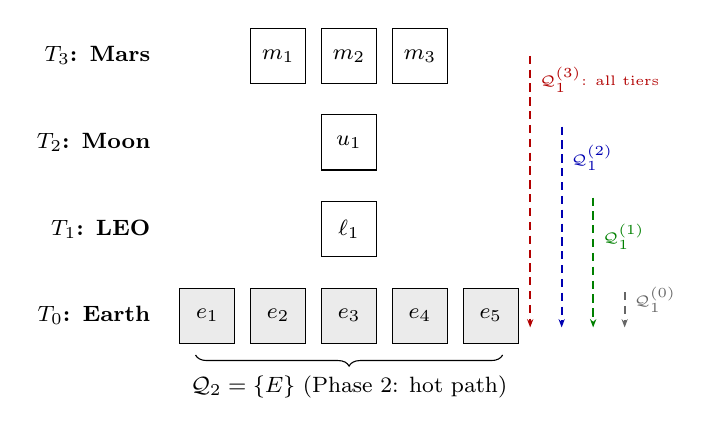
\begin{tikzpicture}[
    node/.style={draw, minimum width=0.7cm, minimum height=0.7cm, font=\footnotesize},
    tierlab/.style={font=\footnotesize\bfseries, anchor=east},
    arrow/.style={-{Stealth[length=3pt]}, thick},
    phase2box/.style={draw, fill=black!8, minimum width=0.7cm, minimum height=0.7cm, font=\footnotesize},
]
% Earth row (tier 0) - 5 nodes
\node[phase2box] (e1) at (0, 0) {$e_1$};
\node[phase2box] (e2) at (0.9, 0) {$e_2$};
\node[phase2box] (e3) at (1.8, 0) {$e_3$};
\node[phase2box] (e4) at (2.7, 0) {$e_4$};
\node[phase2box] (e5) at (3.6, 0) {$e_5$};
\node[tierlab] at (-0.6, 0) {$T_0$: Earth};

% LEO row (tier 1) - 1 node
\node[node] (l1) at (1.8, 1.1) {$\ell_1$};
\node[tierlab] at (-0.6, 1.1) {$T_1$: LEO};

% Moon row (tier 2) - 1 node
\node[node] (u1) at (1.8, 2.2) {$u_1$};
\node[tierlab] at (-0.6, 2.2) {$T_2$: Moon};

% Mars row (tier 3) - 3 nodes
\node[node] (m1) at (0.9, 3.3) {$m_1$};
\node[node] (m2) at (1.8, 3.3) {$m_2$};
\node[node] (m3) at (2.7, 3.3) {$m_3$};
\node[tierlab] at (-0.6, 3.3) {$T_3$: Mars};

% Phase 1 arrows showing "read downward"
% Mars proposer reads all 4 tiers
\draw[arrow, color=red!70!black, densely dashed] (4.1, 3.3) -- node[right, font=\tiny, pos=0.5] {} (4.1, -0.15);
\node[font=\tiny, color=red!70!black, anchor=west] at (4.1, 3.0) {$\mathcal{Q}_1^{(3)}$: all tiers};

% Moon proposer reads 3 tiers
\draw[arrow, color=blue!70!black, densely dashed] (4.5, 2.4) -- (4.5, -0.15);
\node[font=\tiny, color=blue!70!black, anchor=west] at (4.5, 2) {$\mathcal{Q}_1^{(2)}$};

% LEO proposer reads 2 tiers
\draw[arrow, color=green!50!black, densely dashed] (4.9, 1.5) -- (4.9, -0.15);
\node[font=\tiny, color=green!50!black, anchor=west] at (4.9, 1) {$\mathcal{Q}_1^{(1)}$};

% Earth proposer reads 1 tier
\draw[arrow, color=black!60, densely dashed] (5.3, 0.3) -- (5.3, -0.15);
\node[font=\tiny, color=black!60, anchor=west] at (5.3, 0.2) {$\mathcal{Q}_1^{(0)}$};

% Phase 2 brace
\draw[decorate, decoration={brace, amplitude=4pt, mirror}] (-0.15, -0.5) -- (3.75, -0.5)
    node[midway, below=4pt, font=\footnotesize] {$\mathcal{Q}_2 = \{E\}$ (Phase~2: hot path)};
\end{tikzpicture}
\caption{The crumbling-wall construction over the 5/1/1/3 topology. Each tier's Phase~1 quorum reads downward through the wall (dashed arrows). Phase~2 uses only the Earth row (shaded). The wall narrows from bottom to top: wider rows offer more quorum choices.}
\label{fig:wall}
\end{figure}

Let $\mathcal{Q}_1^{(i)}$ denote the Phase~1 family for a proposer at tier~$i$:
\[
\mathcal{Q}_1^{(i)} = \bigl\{Q \subseteq N \;\big|\; \forall\, j \le i:\; Q \cap T_j \neq \emptyset\bigr\}.
\]
A proposer at tier~$i$ needs at least one node from every tier at or below it ($j \le i$). For example, $\mathcal{Q}_1^{(2)}$ (Moon) requires intersection with $T_0$ (Earth), $T_1$ (LEO), and $T_2$ (Moon), which is every tier from Moon down to Earth. For relaxed Phase~2 (Section~\ref{sec:relaxed}), Phase~1 additionally requires enough Earth nodes to satisfy a pigeonhole intersection constraint.

Only the Earth floor is required for Paxos safety. Each additional downward-path witness represents a deployment policy that requires a tier to participate in acquisition---for example local representation, administrative control, sovereignty, or fencing before authority crosses a boundary. If no such policy applies, the extra witness is not justified by consensus itself; in that setting the wall should be read as an analytical construction rather than a recommended deployment geometry.

\subsection{Phase~2 Family}

The Phase~2 family places the hot commit path entirely on the fast tier:
\[
\mathcal{Q}_2 = \{E\}.
\]
That is, Phase~2 requires all five Earth nodes (the strict construction). Section~\ref{sec:relaxed} relaxes this to $k$-of-$|E|$.

\subsection{Safety: Quorum Intersection}

\refstepcounter{prop}\label{prop:intersection}\textbf{Proposition \theprop.} For every tier $i$ and every $Q_1 \in \mathcal{Q}_1^{(i)}$, $Q_2 \in \mathcal{Q}_2$: $Q_1 \cap Q_2 \neq \emptyset$.

\textit{Proof.} Every $\mathcal{Q}_1^{(i)}$ requires $Q_1 \cap T_0 \neq \emptyset$ (since $0 \le i$ for all $i$, i.e., Earth is at or below every tier). $Q_2 = E = T_0$. Therefore $Q_1 \cap Q_2 \supseteq Q_1 \cap T_0 \neq \emptyset$. \hfill $\square$

The intersection follows from the wall's structure: every path through the wall reaches the bottom row, and Phase~2 is the bottom row.

We verified this mechanically in TLA+. For readers who have not used it: TLA+ is a specification language whose model checker, TLC, enumerates \emph{every} state reachable from the initial conditions of a finite model and checks the stated invariant in each one. A run is \emph{complete} when that enumeration reaches a fixed point---no reachable state was left unexamined---so a complete run is a proof of the invariant for that finite model, not a statistical sample of behaviors. The \texttt{QuorumIntersection} specification enumerates every (construction $\times$ initiating tier $\times$ $Q_1$ $\times$ $Q_2$) combination for the strict, $k{=}4$, and $k{=}3$ families over the full 10-node topology (27{,}921 states, complete); \texttt{ExhaustiveIntersection} re-checks the strict and $k{=}4$ families as parse-time assumptions. No intersection failure was found.

For the full Paxos protocol (not just quorum intersection), we verify safety over a reduced 6-node topology ($3E + 1L + 1U + 1M$) that preserves the quorum-intersection structure. The invariant the reduction preserves is the pigeonhole inequality, not tier membership alone: in the reduced model both quorum families guarantee at least two of the three Earth nodes ($2 + 2 > 3$), and in the full modeled family $Q_1$ carries at least two Earth nodes against a 4-of-5 $Q_2$ ($2 + 4 > 5$)---both instantiate $|Q_1 \cap E| \ge |E| - k + 1$ with the margin $|E| - k = 1$ held fixed. (Tier membership alone suffices only under strict $\mathcal{Q}_2 = \{E\}$, where any Earth node in $Q_1$ intersects it.) Liveness properties (crash tolerance, progress under partial failure) are topology-size-dependent and are evaluated only at full scale. Over the reduced topology, single-decree Paxos agreement was model-checked completely (67M~states, no violation).

\textbf{Verification scope.} The protocol-level specification models a single all-tier Phase~1 family rather than the per-tier families of Section~\ref{sec:construction}: it exercises the protocol machinery under wall-shaped quorums, but safety of the per-tier construction itself rests on Proposition~\ref{prop:intersection} and the standard Flexible Paxos argument, with the intersection premise checked exhaustively above. The proof is primary; the model checking is corroboration. Specifications are in \texttt{tla/} (see \autoref{app:traceability}).

\subsection{Liveness: Reading the Wall}
\label{sec:liveness-wall}

The wall determines liveness as follows. A proposer at tier~$i$ can complete Phase~1 if and only if it can reach at least one node in every tier~$j$ where $j \le i$ (from its own tier down to Earth). Phase~2 succeeds if the proposer can reach enough Earth nodes (all five under strict $\mathcal{Q}_2$).

During Mars conjunction blackout, cross-tier links between Mars and the inner system are removed: Mars is partitioned from Moon, LEO, and Earth, while those three remain mutually connected. Reading the wall against that connectivity takes one pass per tier. Earth needs only $T_0$ and is trivially satisfied; LEO needs $T_0$ and $T_1$; Moon needs $T_0$ through $T_2$; all three are reachable, so all three work. Mars needs a witness from every tier including the inner ones it cannot reach, and is blocked. The liveness failure is scoped to exactly the disconnected tier: the wall crumbles from the top (Figure~\ref{fig:blackout}).

\begin{figure}[t]
\centering
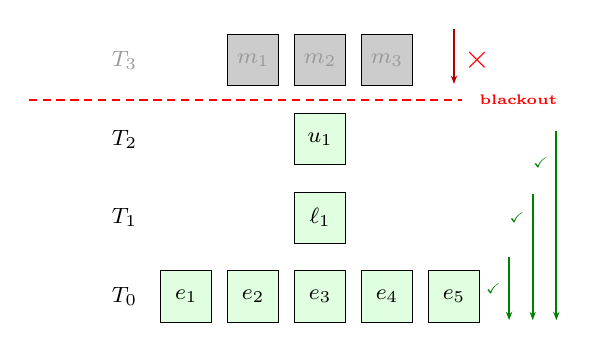
\begin{tikzpicture}[
    node/.style={draw, minimum width=0.65cm, minimum height=0.65cm, font=\footnotesize},
    dead/.style={draw, minimum width=0.65cm, minimum height=0.65cm, font=\footnotesize, fill=black!20, text=black!40},
    ok/.style={draw, minimum width=0.65cm, minimum height=0.65cm, font=\footnotesize, fill=green!12},
    tierlab/.style={font=\footnotesize\bfseries, anchor=east},
    arrow/.style={-{Stealth[length=3pt]}, thick},
]
% Earth row
\node[ok] (e1) at (0, 0) {$e_1$};
\node[ok] (e2) at (0.85, 0) {$e_2$};
\node[ok] (e3) at (1.7, 0) {$e_3$};
\node[ok] (e4) at (2.55, 0) {$e_4$};
\node[ok] (e5) at (3.4, 0) {$e_5$};
\node[tierlab] at (-0.5, 0) {$T_0$};

% LEO row
\node[ok] (l1) at (1.7, 1.0) {$\ell_1$};
\node[tierlab] at (-0.5, 1.0) {$T_1$};

% Moon row
\node[ok] (u1) at (1.7, 2.0) {$u_1$};
\node[tierlab] at (-0.5, 2.0) {$T_2$};

% Mars row - grayed out
\node[dead] (m1) at (0.85, 3.0) {$m_1$};
\node[dead] (m2) at (1.7, 3.0) {$m_2$};
\node[dead] (m3) at (2.55, 3.0) {$m_3$};
\node[tierlab, text=black!40] at (-0.5, 3.0) {$T_3$};

% Partition line
\draw[thick, red, densely dashed] (-2.0, 2.5) -- (3.5, 2.5);
\node[font=\tiny\bfseries, color=red, anchor=west] at (3.6, 2.5) {blackout};

% Working paths
\draw[arrow, color=green!50!black] (4.1, 0.5) --  (4.1, -0.3);
\node[font=\tiny, color=green!50!black] at (3.9, 0.1) {$\checkmark$};
\draw[arrow, color=green!50!black] (4.4, 1.3) -- (4.4, -0.3);
\node[font=\tiny, color=green!50!black] at (4.2, 1) {$\checkmark$};
\draw[arrow, color=green!50!black] (4.7, 2.1) -- (4.7, -0.3);
\node[font=\tiny, color=green!50!black] at (4.5, 1.7) {$\checkmark$};

% Blocked path
\draw[arrow, color=red!70!black] (3.4, 3.4) -- (3.4, 2.7);
\node[font=\large, color=red] at (3.7, 3) {$\times$};
\end{tikzpicture}
\caption{Liveness under Mars conjunction blackout. The partition (dashed line) disconnects $T_3$. Earth, LEO, and Moon can still read downward to form Phase~1 quorums (green arrows). Mars cannot reach any inner tier (red $\times$). The wall crumbles from the top.}
\label{fig:blackout}
\end{figure}

This instantiates the legibility definition of Section~1: for any tier~$i$, global Phase~1 succeeds if and only if every tier~$j \le i$ is reachable from~$i$ in~$C$---the promised $O(\text{tiers})$ check. This is what distinguishes legibility from mere computability. The claim concerns quorum formability: it bounds what a sole, timely proposer can achieve under connectivity state $C$, and does not speak to contention between concurrent proposers, whose durable promises can delay an otherwise-capable peer. Global \emph{operation}, as opposed to Phase~1 recovery, additionally requires the Phase~2 quorum to be reachable; Section~\ref{sec:reachability} shows the two conditions coming apart.

\subsection{Capability Gaps in the Wall}
\label{sec:capability-wall}

Section~\ref{sec:capability} defines the two formability predicates for an arbitrary pair of quorum families. The wall instantiates them per tier: write $R_1(i,C)$ when $C \in \operatorname{Form}(\mathcal{Q}_1^{(i)})$ and $R_2(i,C)$ when $C \in \operatorname{Form}(\mathcal{Q}_2)$, so every tier carries its own acquisition predicate against one shared commit predicate. Which gaps are reachable is therefore a per-tier question, and the answer is not uniform across tiers.

\refstepcounter{prop}\label{prop:boundary}\textbf{Proposition \theprop\ (boundary).} For the construction of Section~\ref{sec:construction} under relaxed $\mathcal{Q}_2 = k$-of-$|E|$ (Section~\ref{sec:relaxed}), $(1,0)$ is unreachable at \emph{every} tier if and only if $|E| - k + 1 \ge k$, that is $k \le \lceil |E|/2 \rceil$. Sufficiency is unconditional---it does not depend on the number of tiers, their sizes, or the initiating tier. The converse additionally requires non-degeneracy: no empty wall row.

The arithmetic is the same hitting-set bound that carries safety. A $Q_1$ holds at least $|E|-k+1$ Earth nodes and a $Q_2$ holds $k$; when $|E|-k+1 \ge k$, every $Q_1$ already contains a full $Q_2$ and Proposition~\ref{prop:gap} applies.

\textbf{The gradient.} Proposition~\ref{prop:boundary} governs $(1,0)$ through the Earth floor. It says nothing about $(0,1)$, which on this construction arises from a different mechanism: the downward chain. A proposer at $T_2$ (Moon) needs one witness from $T_1$ (LEO), and this topology has exactly one LEO node. Sever it while all five Earth nodes remain reachable and $\mathcal{Q}_2$ is formable while $\mathcal{Q}_1^{(2)}$ is not. Exhaustive enumeration over all $2^{10}$ connectivity states, for every tier and every $k$, gives:

\begin{center}
\begin{tabular}{@{}lcccc@{}}
\toprule
 & $T_0$ (E) & $T_1$ (L) & $T_2$ (U) & $T_3$ (M) \\
\midrule
$(1,0)$ reachable & $k \ge 4$ & $k \ge 4$ & $k \ge 4$ & $k \ge 4$ \\
$(0,1)$ reachable & $k \le 2$ & $k \le 2$ & all $k$ & all $k$ \\
\bottomrule
\end{tabular}
\end{center}

Read the two rows together: \emph{no value of $k$ closes both states}. At $k \le 2$ the Earth floor exceeds $k$ and every tier carries $(0,1)$ exposure. At $k \ge 4$ Proposition~\ref{prop:boundary}'s bound is violated and $(1,0)$ opens everywhere. At $k = 3$---the best available configuration, and the relaxation Section~\ref{sec:relaxed} adopts---$(1,0)$ is closed at every tier and $(0,1)$ is closed at Earth and LEO, but Moon and Mars retain it. Those are exactly the tiers with an intervening row between themselves and the anchor, and no choice of $k$ removes it, because the obligation that fails is a witness row rather than an Earth count.

The enumeration credits each proposer with a reachable node in its own tier, modelling a colocated acceptor; without that assumption LEO also retains $(0,1)$ at every $k$, since its single node can be severed while Earth remains whole. We state the assumption rather than absorb it: it determines whether phase symmetry is affordable at one tier or two.

\textbf{Relationship to Flexible Paxos.} The $(1,0)$ state is not new, and the Flexible Paxos paper describes it twice~\cite{howard2016}: once in the $|Q_1|{=}1$, $|Q_2|{=}N$ construction, and once in the row-failure discussion, where completing $Q_1$ ``recover[s] all past decisions'' before falling back to reconfiguration. Both readings are constructive, and our measurements agree with them (Section~\ref{sec:valence}). Our relationship to that work is therefore threefold. It identifies the state and a use for it; we supply the design-time existence criterion---for a given construction, whether the state arises at all, which FPaxos \S4.3 does not ask; and we find that the cost, where it exists, lies in the unexamined dual. What FPaxos \S4.3 assumes is available and the connectivity setting does not supply is a \emph{recognizer}: its prescribed response presumes the system knows which state it occupies. Under a known crash-failure set that is reasonable. Under connectivity it is exactly the missing predicate, and supplying it is what the readout of Section~\ref{sec:liveness-wall} does.

This is the sense in which legibility is load-bearing rather than decorative. The gradient is not an artifact we can relax away; it is a property of any wall whose non-anchor rows carry witness obligations. When a capability gap cannot be closed by construction, state-aware mitigation requires distinguishing the state. The connectivity data needed is already available to an operator; what was missing was the predicate that reads it. Enumeration and auditor artifacts are in \texttt{results/capability/} (see \autoref{app:traceability}).

The wall-specific capability readout turns that predicate into a small operational interface. Given named tiers, a Phase~2 threshold, an initiating tier, a reachable-node summary, and the provenance of both configuration and connectivity, it reports $(R_1,R_2)$, quorum witnesses, and typed failed obligations. It deliberately reports runtime authority as unknown and service policy as not inferred. The planetary and terrestrial-edge inputs are a demonstration artifact, not empirical evidence.

\subsection{What ``Global'' Means}

When an Earth-based proposer completes both phases using only Earth nodes, the decision is \emph{global} in the Paxos sense: any future proposer at any tier, upon completing Phase~1, will discover this value in the Earth acceptors' state and cannot contradict it. Global consensus does not require that all tiers participated, only that no future quorum can produce a conflicting result.


\section{Related Work}

Paxos established the standard safety argument for replicated state machines under asynchronous messaging and crash failures~\cite{lamport1998}. Flexible Paxos showed that safety requires only Phase~1/Phase~2 cross-intersection, not universal majority~\cite{howard2016}. Our characterization builds on that result but does not claim containment itself as a new mathematical tool. The contribution is the exact correspondence between phase-formability ordering and its complete gap profile, the operational interpretation of those gaps, and their application to phase-asymmetric Paxos.

Containment has important prior uses. Refined Quorum Systems~\cite{guerraoui2010rqs} nests quorum classes $QC_1 \subseteq QC_2 \subseteq RQS$ to connect resilience with optimistic complexity, subject to adversary-aware intersection properties. That class inclusion is a design and correctness condition, not an ordering of two phase-formability predicates over connectivity states. Li, Chan, and Lesani's quorum subsumption~\cite{li2023} is a member-indexed containment condition: for every process $p$ in a quorum $q$, some quorum in $p$'s personal family is contained in $q$. It supports progress in a heterogeneous Byzantine trust model. We instead compare two phase predicates over one fixed crash-stop acceptor universe. The quantifiers and the questions differ even though both results use containment.

Grid and crumbling-wall quorum constructions~\cite{cheung1992,peleg1995} demonstrate that quorum geometry can be engineered around combinatorial structure. Howard et al.\ note explicitly that Flexible Paxos can use such constructions; we take up that suggestion. Peleg and Wool analyzed crumbling-wall availability under random, independent node failures. Our wall case study maps rows to physical latency tiers and examines per-tier liveness under scheduled, topology-correlated disconnection. Its upper-tier witnesses are useful only when participation policy requires local representation, administrative control, sovereignty, or fencing; absent such a requirement, the wall remains an analytical example rather than recommended deployment geometry. Li, Chan, and Lesani's Satrapy system~\cite{li2026satrapy} carries heterogeneous quorum theory into practical consensus. Hierarchical quorum structures have a longer history in database replication~\cite{daudjee2004} and coordination services; our wall differs in that the hierarchy reflects physical latency tiers rather than organizational or logical grouping.

Geo-distributed consensus provides the closest practical analog. WPaxos~\cite{ailijiang2019wpaxos} uses Flexible Paxos with grid quorum layouts and per-object multi-leader coordination to keep commits local; it is the nearest point of comparison. WPaxos's grid quorums are symmetric: $Q_1$ spans $Z - f_z$ zones and $Q_2$ spans $f_z + 1$ zones, with the same structure regardless of which node initiates. Our per-tier $\mathcal{Q}_1^{(i)}$ families are asymmetric as the initiating tier determines the quorum scope, which produces a leadership cost gradient that symmetric grids structurally cannot express (Section~\ref{sec:discussion}). EPaxos~\cite{moraru2013} removes the leader bottleneck for non-conflicting commands. Mencius~\cite{mao2008} distributes leader responsibility across WAN sites. MDCC~\cite{kraska2013} achieves single-round cross-datacenter commits. All four optimize for tens-to-hundreds of milliseconds WAN latency and assume all replicas are usually reachable. Our setting differs in two respects: the asymmetry spans three orders of magnitude (sub-second to 1342~s), and the target phenomenon is scheduled total disconnection rather than heterogeneous latency.

Delay-tolerant networking~\cite{cerf2007,fall2003} motivates the operating regime but addresses routing and custody transfer, not consensus. CRDTs have been studied in DTN-like settings~\cite{guidec2023}. SwarmDAG~\cite{tran2019swarmdag} uses extended virtual synchrony for partition-tolerant robot swarms; Tran et al.~\cite{tran2019milcom} measure consensus latency under partitioning. Protocol Labs' IPC~\cite{delarocha2022} uses hierarchical subnets for blockchain scaling. NASA's DSN study~\cite{connell2011} evaluates database replication for ground stations. Our work occupies a gap: Paxos safety under topology-shaped quorum geometry and scheduled disconnection, with per-tier liveness characterization.


\section{Experimental Design}
\label{sec:expdesign}

Eidolon is a discrete-event simulator built on SimPy. Acceptors process Prepare and Accept messages with configurable processing delay. Proposers fan out messages to all acceptors and collect responses with a per-phase timeout. The network model assigns entities to named locations with per-link latency, jitter, and optional loss. Blackout is modeled as deterministic link removal; the repeater model substitutes a degraded alternate path. Event ordering is by simulation timestamp; the simulator is deterministic given a seed.

\subsection{Topology}

Five Earth ground stations (NA-West, Europe, Asia, SA-East, Africa) with cross-continental latencies of 30--120~ms. One LEO satellite with 20--45~ms links to ground stations. One Moon node at 1.28~s one-way. Three Mars nodes at configurable one-way delay (186--1342~s, representing closest approach to opposition). Mars-local links are 5~ms.

We evaluate two network variants:
\begin{itemize}
\item \textbf{Sparse}: LEO has links to 3 of 5 Earth stations (NA-West, Europe, Asia). Mars has links to 2 of 5 (NA-West, Europe). This models a single LEO satellite with limited ground coverage and a Mars relay with two tracking stations.
\item \textbf{Full coverage}: LEO and Mars have links to all 5 Earth stations. This models a LEO constellation with global coverage and a deep-space network with worldwide antenna placement.
\end{itemize}

\subsection{Experiments}

Four experiment families probe different aspects of the construction; the fourth, the pre-registered valence experiment, is described with its results in Section~\ref{sec:valence}.

\begin{table}[t]
\centering
\small
\caption{Experimental design.}
\label{tab:design}
\footnotesize
\begin{tabular}{>{\raggedright\arraybackslash}p{0.16\linewidth}>{\raggedright\arraybackslash}p{0.30\linewidth}>{\raggedright\arraybackslash}p{0.34\linewidth}}
\toprule
Experiment & Purpose & Key parameters \\
\midrule
Parameter sweep & Confirm structural invariance of Earth-initiated global consensus across Mars delay and blackout duration & Mars delay $\in \{186, 750, 1342\}$~s; blackout $\in \{300, 900, 1800\}$~s; 50 seeds per point \\
Per-tier sweep & Measure which tiers retain global liveness; compare sparse vs.\ full-coverage topologies & Initiating tier $\in \{$Mars, Moon, LEO, Earth$\}$; both topologies; 186~s Mars delay; 900~s blackout; 50 seeds \\
Crash tolerance & Characterize the tradeoff between Phase~2 relaxation ($k$-of-$|E|$) and crash tolerance & $k \in \{3, 4, 5\}$; 0--2 Earth crashes; 186~s; 900~s blackout; 50 seeds \\
\bottomrule
\end{tabular}
\end{table}

Fixed parameters across all experiments are listed in Table~\ref{tab:params} (\autoref{app:params}). All seeds are 40--89 (50 runs per point). Results are reported as means with 95\% confidence intervals.


\section{Results}
\label{sec:results}

\subsection{The Valence of the Two Capability States}
\label{sec:valence}

Section~\ref{sec:capability} says when each state arises. It does not say what either costs, and the two turn out to cost very different things. We registered predictions, a falsification criterion, and the consequence of a null before the experiment existed. The registered suspect was the intuitive one---an incumbent able to win ballots it cannot use, standing between healthy proposers and progress---and we predicted it would degrade their outcomes. That prediction was falsified in the opposite direction from the one expected, and we report it as registered.

The setting is single-decree Paxos. A healthy proposer competes with an incumbent whose capability state is set by a mid-round connectivity change, with the retry budget swept over $\{1, 2, 4, 8\}$ and 50 seeds per cell. The incumbent sits at the Moon tier, since an Earth-tier proposer is colocated with an Earth acceptor and no partition can fail its Phase~1 while leaving Earth reachable. The experiment exists only at $k{=}5$: by Proposition~\ref{prop:boundary}, at $k \le 3$ there is no $(1,0)$ state to place an incumbent into.

\begin{center}
\setlength{\tabcolsep}{4pt}
\begin{tabular}{@{}lcccc@{}}
\toprule
Incumbent state & $P(\text{ok})$ & med.\ ttfc & rounds & NACKs \\
\midrule
$(1,0)$, flip-induced & 1.000 & 3.420~s & 2 & 7 \\
$(1,1)$, fully healthy & 1.000 & 3.420~s & 2 & 7 \\
$(0,1)$ & 0.000 & --- & --- & 48--49 \\
\bottomrule
\end{tabular}
\end{center}

The first two rows are the result. A $(1,0)$ incumbent is metric-for-metric indistinguishable from a perfectly healthy competing proposer, at every retry budget, on every column we recorded. Whatever a $(1,0)$ incumbent costs the system, an ordinary contending peer costs exactly the same: the cost is contention, not the capability state. Its arm is also flat in the retry budget while its own Phase~1 completions climb from 1 to 8. The third row is the state nobody examined: at retry budget~8 the healthy proposer fails in 50 of 50 seeds, with Wilson intervals disjoint from the row above. Where the $(0,1)$ state is placed within the round does not matter---early and late placements overlap at every budget.

\textbf{Mechanism: failure is cheap, success is expensive.} A proposer that fails Phase~1 learns so immediately and retries after a short backoff. A proposer that \emph{completes} Phase~1 and then cannot form $\mathcal{Q}_2$ must wait a full phase timeout before it can try again. It is throttled by its own success. The policy-independent core is that completing a phase imposes a floor on the retry interval---at least one phase timeout, which must exceed the round trip---while failing a phase imposes no floor at all. How small the floor-free cycle is depends on the backoff policy, which we deliberately do not study; the existence of the asymmetry does not.

Two things this is not. The observed blocking is exhaustion of a bounded retry budget, not livelock: we make no livelock claim. And the $(1,0)$ result is not merely an absence of harm. Its partial Phase~2 reaches four of the five Earth acceptors; the next proposer's Phase~1 surfaces that accepted value, and ordinary Paxos value adoption carries it to commitment. The $(1,0)$ proposer is a value injector rather than a spoiler, which is the constructive reading of Flexible Paxos \S4.3 observed with its mechanism visible.

\textbf{Scope.} Under Multi-Paxos a $(0,1)$ tier keeps committing while its authority survives, deferring exposure to the moment authority must be re-acquired; under single-decree every decree needs Phase~1, so the block is immediate. The measured setting is the severe one.

\textbf{Deviations, recorded.} Five, with reasons, in the artifact record alongside the verdict table and threats: the flip lands before Phase~2 fan-out rather than in its return leg, which would test acknowledgment loss instead of a capability state; the intended $(0,0)$ control was realized as $(0,1)$, the only state failing Phase~1 while still reaching the anchor; and one arm was added because the registered timing prediction was untestable as written.

\subsection{Flat versus Crumbling Wall: Geometry Alone Changes the Outcome}

To calibrate the effect of quorum geometry, we compare three constructions over the identical topology, blackout model, and parameter sweep. The \emph{flat} construction uses a single Phase~1 family requiring all four tiers:
\[
\mathcal{Q}_1^{\text{flat}} = \bigl\{Q \subseteq N \;\big|\; \forall\, j \in \{0,1,2,3\}:\; Q \cap T_j \neq \emptyset\bigr\}.
\]
Any blackout that removes a tier makes this quorum unformable. The \emph{majority} baseline is a competitive shape-free Flexible Paxos configuration: $\mathcal{Q}_1^{\text{maj}} = \{Q \mid |Q| \ge 6\}$, any majority of the ten nodes, with no tier structure. The \emph{crumbling wall} construction uses the per-tier Phase~1 families defined in Section~\ref{sec:construction}, with an Earth-based global proposer. All three satisfy cross-intersection with $\mathcal{Q}_2 = \{E\}$: the tiered families require $Q_1 \cap T_0 \neq \emptyset$ directly, and any 6 of 10 nodes must include an Earth node because only five non-Earth nodes exist.

\begin{table}[t]
\centering
\small
\caption{Effect of quorum geometry: flat vs.\ majority vs.\ crumbling-wall Phase~1 over the same topology and blackout model. Earth-initiated global proposer, hard blackout, 50 seeds per point; rates are identical at all 9 parameter points (3 Mars delays $\times$ 3 blackout durations). Latency is the full two-phase (Phase~1 $+$ Phase~2) decision latency of a single attempt.}
\label{tab:flat-vs-wall}
\begin{tabular}{p{0.40\linewidth}rrr}
\toprule
Construction & During & Post & Latency \\
\midrule
Flat Phase~1 (all tiers required) & 0.0\% & varies & varies \\
Majority Phase~1 (any 6 of 10) & 100.0\% & 100.0\% & 0.361~s \\
Crumbling wall (Earth reads Earth only) & 100.0\% & 100.0\% & 0.183~s \\
\bottomrule
\end{tabular}
\end{table}

The flat construction yields 0\% during-blackout success at every sweep point because it requires all tiers, including disconnected Mars. The crumbling wall yields 100\% because the Earth-based proposer's Phase~1 reads only Earth. Zero variance across 50 seeds confirms that outcomes here are structural consequences of quorum geometry and link state, not scheduler artifacts. We therefore treat this as calibration, not discovery.

The majority baseline separates what the wall's geometry buys from what any sufficiently slack quorum buys. Majority Phase~1 also sustains 100\% during-blackout success for the Earth-initiated proposer: the blackout removes three nodes and a 6-of-10 quorum tolerates four, so blackout survival here is within the slack of a shape-free quorum. What the geometry changes is everything else. Two-phase decision latency doubles (0.361~s vs.\ 0.183~s, uniformly across the sweep): the sixth-fastest respondent lies outside Earth, so majority Phase~1 leaves the fast tier even when nothing has failed. Both constructions share the identical all-Earth Phase~2, so steady-state Multi-Paxos commits do not differ; the penalty falls on authority acquisition, recovery, and single-decree decisions---every operation that pays Phase~1. The tolerance is not tier-aware: during blackout a LEO-initiated proposer reaches only five acceptors (itself, three ground stations, and Moon), so majority Phase~1 is unformable from LEO while the wall's LEO family still completes Phase~1. And the valid-quorum count collapses to a single tier-independent value ($\sum_{k \ge 6} \binom{10}{k} = 386$), below Earth's 992 wall quorums and without the per-tier gradient of Figure~\ref{fig:gradient}. The wall's contribution over a well-chosen flexible quorum is therefore not raw blackout survival, which slack alone can purchase; it is what slack cannot express---Phase~1 kept inside the fast tier, per-tier legibility of degradation, and the leadership gradient of Section~\ref{sec:discussion}.

\subsection{Per-Tier Liveness: The Wall Crumbles from the Top}

Table~\ref{tab:pertier} reports the central result. Under full network coverage, each tier runs its own global proposer during Mars conjunction blackout (186~s one-way, 900~s blackout, hard blackout model, 50 seeds).

\begin{table}[t]
\centering
\small
\caption{Per-tier global consensus during Mars conjunction blackout (full-coverage topology, hard blackout, 186~s Mars delay, 900~s blackout, mean $\pm$ 95\% CI over 50 seeds). Rates are identical across seeds (structural outcomes; no CIs shown); recovery lags are cadence artifacts (see text). $^{\dagger}$Undefined: no Mars attempt lies wholly within this window (see text).}
\label{tab:pertier}
\begin{tabular}{llrrr}
\toprule
Tier & Position & During & Latency & Rec.\ lag \\
\midrule
Earth & bottom (0) & 100.0\% & 0.183~s & 68.1~s \\
LEO & tier 1 & 100.0\% & 0.131~s & 67.2~s \\
Moon & tier 2 & 100.0\% & 5.131~s & 27.1~s \\
Mars & top (3) & ---$^{\dagger}$ & 752.5~s & 1009.3~s \\
\bottomrule
\end{tabular}
\end{table}

Three of four tiers retain global consensus capability during hard Mars blackout. Only Mars, which is the disconnected tier, loses it. The liveness failure crumbles from the top of the wall, exactly as the construction predicts. (95\% CIs: latency within $\pm 0.001$~s and recovery lag within $\pm 0.01$~s for Earth, LEO, and Moon; $\pm 0.7$~s and $\pm 1.7$~s for Mars.)

The latency column maps directly to physics. Moon's 5.131~s is two Paxos phases at the 1.28~s one-way Moon--Earth light delay ($\approx 4 \times 1.28$~s). Earth's 183~ms reflects cross-continental round-trips within the Earth tier. LEO's 131~ms is \emph{faster} than Earth, which is a counterintuitive result explained by the network topology: LEO-to-ground links (20--45~ms) are shorter than cross-continental Earth links (50--120~ms). Wall position determines quorum \emph{obligations}; the speed of light determines their \emph{cost}. These are correlated but not identical, and LEO is the proof.

Mars fails during blackout for the structural reason predicted by the wall (it cannot reach inner tiers for Phase~1). At the table's 900~s point, however, no Mars attempt lies wholly within the blackout---a failed attempt occupies one 500~s Phase~1 timeout, and the attempt cadence, phase-shifted by the long pre-blackout round, straddles the boundary---so the during-blackout cell is undefined rather than zero. The prediction is observed directly at the 1800~s blackout duration, where the cadence places complete failed attempts inside the window: during-blackout success is 0\% across all 50 seeds. Outside blackout, however, Mars-initiated global consensus \emph{succeeds}: every pre- and post-blackout attempt completes across all 50 seeds, at a mean latency of 752.5~s---two Paxos phases at the 186~s one-way Mars--Earth delay ($\approx 4 \times 186$~s). Success requires a per-phase timeout budget sized to the initiating tier's physics: the worst-case request--response path from Mars is $2 \times 186 \approx 372$~s, within the 500~s per-phase budget of Table~\ref{tab:params}. This is not a blackout finding but a physics finding: Mars-initiated global consensus is possible but pays the full interplanetary round trip on every phase, so in practice delegation to a lower-tier proposer dominates.

Recovery lag differences between tiers (27.1~s for Moon vs.\ 68.1~s for Earth) are cadence-alignment artifacts, not protocol properties. Recovery lag measures the gap from blackout end to the next successful cadence-aligned attempt, so it is quantized by the 120~s reconciliation interval: its value is bounded by one interval plus a round time, and where it falls within that bound depends only on where the blackout boundary lands in each tier's attempt cadence.\footnote{Each tier's per-round time shifts its cadence phase relative to blackout end, which is why the values differ across tiers and move when the experiment window shifts. The effect is deterministic and independent of the consensus protocol; the bound, not the value, is the protocol property.}


\subsection{Wall Obligations versus Network Reachability}
\label{sec:reachability}

Table~\ref{tab:sparse} repeats the per-tier experiment under the sparse network topology.

\begin{table}[t]
\centering
\small
\caption{Per-tier global consensus under sparse topology (same parameters as Table~\ref{tab:pertier}). All rates are identical across the 50 seeds---structural outcomes, reported without CIs.}
\label{tab:sparse}
\begin{tabular}{llr}
\toprule
Initiating tier & Wall prediction & Sparse result \\
\midrule
Earth & works & 100.0\% \\
LEO & works & 0.0\% \\
Moon & works & 100.0\% \\
Mars & blocked & 0.0\% \\
\bottomrule
\end{tabular}
\end{table}

LEO drops from 100\% (full coverage) to 0\% (sparse). The wall says LEO needs LEO $+$ Earth; that obligation is satisfiable. But strict Phase~2 requires all five Earth nodes, and LEO has links to only three ground stations. The wall determines what a tier \emph{needs}; the network determines what it \emph{can reach}. Liveness requires both.

This makes legibility a two-step operator procedure: check the wall structure (which determines quorum obligations per tier) and check the network topology (which determines whether those obligations are achievable). The wall is the blueprint; the network is the building site.

Moon succeeds in both topologies because it has links to all five Earth ground stations. The sparse topology models a single LEO satellite with limited ground coverage; the three missing ground-station links are the difference between 0\% and 100\% for LEO-initiated consensus.


\section{Crash Tolerance and Coordinated Relaxation}
\label{sec:relaxed}

The strict Phase~2 choice $\mathcal{Q}_2 = \{E\}$ introduces a fragility: a single crashed Earth acceptor blocks all global Phase~2 progress. This section relaxes that choice.

\subsection{Relaxed Construction}
Let the relaxed Phase~2 family require $k$ of $|E|$ Earth nodes. We evaluate $k = 4$ (tolerates one crash) and $k = 3$ (tolerates two). Phase~1 requires correspondingly more Earth nodes to maintain intersection: a $k$-of-$|E|$ Phase~2 quorum omits at most $|E| - k$ Earth nodes, so any set of $|E| - k + 1$ Earth nodes intersects every Phase~2 quorum (pigeonhole). Phase~1 must therefore contain at least $|E| - k + 1$ Earth nodes. For $k = 4$ out of 5 Earth nodes, this means at least 2 Earth nodes in every $Q_1$; for $k = 3$, at least 3. Both relaxed constructions are verified exhaustively in TLA+ alongside the strict one (Section~\ref{sec:construction}).

The relaxed Phase~1 family for tier~$i$ is:
\[
\mathcal{Q}_{1,k}^{(i)} = \bigl\{Q \subseteq N \;\big|\; \forall\, j \le i:\; Q \cap T_j \neq \emptyset,\; |Q \cap E| \ge |E| - k + 1\bigr\}.
\]

\subsection{Results: The Weakest Link Migrates}
Table~\ref{tab:relaxed} reports the crash-tolerance sweep (Earth-initiated, repeater-assisted, 186~s Mars delay, 900~s blackout, 50 seeds).

\begin{table*}[t]
\centering
\small
\caption{Coordinated relaxation under Earth crashes (mean $\pm$ 95\% CI, 50 seeds). Earth-local Flexible Paxos: ``std'' is $q_1{=}4, q_2{=}2$; ``maj'' is $q_1{=}q_2{=}3$. Recovery is the lag from blackout end to the next successful global attempt and is quantized by the 120~s reconciliation cadence (Section~\ref{sec:results}).}
\label{tab:relaxed}
\begin{tabular}{llrrrrr}
\toprule
Global $\mathcal{Q}_2$ & Local & Crashes & Earth-local & Global during & Global post & Recovery (s) \\
\midrule
strict & std & 0 & 100.0\% & 100.0\% & 100.0\% & 93.11$\pm$0.01 \\
strict & std & 1 & 100.0\% & 0.0\% & 0.0\% & n/a \\
4-of-5 & std & 0 & 100.0\% & 100.0\% & 100.0\% & 94.27$\pm$0.01 \\
4-of-5 & std & 1 & 100.0\% & 100.0\% & 100.0\% & 94.26$\pm$0.01 \\
3-of-5 & std & 2 & 60.5\% & 100.0\% & 100.0\% & 94.64$\pm$0.01 \\
3-of-5 & maj & 2 & 100.0\% & 100.0\% & 100.0\% & 94.63$\pm$0.01 \\
\bottomrule
\end{tabular}
\end{table*}

\textbf{Strict Phase~2 is completely crash-intolerant.} A single Earth crash produces permanent global liveness loss (row~2).

\textbf{The weakest link migrates.} At two crashes with standard Earth-local quorums, the \emph{global} construction ($k=3$) maintains 100\% during-blackout success but the \emph{Earth-local} construction loses liveness outright: it cannot form a Phase~1 quorum of 4 with only 3 remaining Earth nodes, so every attempt after the crashes land fails, and the 60.5\% aggregate rate reflects only attempts completed before the crashes (rows~5--6). The global construction's advantage is not that it spans more nodes---for the Earth-initiated proposer used here, both phases of the relaxed global construction touch only Earth nodes---but that its Earth requirements are smaller: at $k=3$, both global phases need only the three surviving Earth nodes, while the Earth-local configuration still demands four. The structural insight is the legibility of the migration: which crashes matter depends on which quorum family's requirements they intersect, and the wall makes each family's requirements explicit.

\textbf{Coordinated relaxation restores resilience.} Relaxing the Earth-local quorum to majority ($q_1 = q_2 = 3$) restores 100\% local success with no loss of global success (row~6). The tradeoff curve, with Phase~1 minima shown for the bottom-initiated (Earth) and top-initiated (Mars) proposers:

\begin{center}
\small
\setlength{\tabcolsep}{3.5pt}
\begin{tabular}{lrrrl}
\toprule
Regime & P1 min E/M & P2 & Tol. & E-local $\mathcal{Q}_2$ \\
\midrule
Strict ($k = 5$) & 1 / 4 & 5-of-5 & 0 & 2-node E \\
Relaxed ($k = 4$) & 2 / 5 & 4-of-5 & 1 & 2-node E \\
Relaxed ($k = 3$) + maj & 3 / 6 & 3-of-5 & 2 & 3-node E \\
\bottomrule
\end{tabular}
\end{center}
An Earth-initiated $Q_1$ needs only the $|E|-k+1$ Earth nodes; a Mars-initiated $Q_1$ adds one witness from each of the three upper tiers. Relaxation buys crash tolerance by growing the cold path, never the hot one: Phase~2 shrinks as Phase~1's Earth requirement grows.


\section{Threats to Validity and Limitations}

All results are design-level, not deployment-level.

\textbf{Anchor concentration.} The wall concentrates both safety and liveness at the bottom row. Every Phase~1 reads down to Earth; every Phase~2 is on Earth. In our construction, this concentration is sufficient for the legibility property: per-tier liveness determination is $O(\text{tiers})$ because a fixed reference point for cross-intersection eliminates the need to enumerate quorum subsets. Distributing the anchor across multiple rows would require reasoning about which row combinations provide intersection---structured multi-anchor families might remain efficiently analyzable, but the wall's simple linear readout would be lost. The single anchor is what makes the wall readable at a glance. Note, however, that the anchor is a \emph{tier}, not a node. Since safety depends only on tier membership (Section~\ref{sec:construction}), the anchor tier's internal replication is unconstrained by the wall---it can be scaled, geo-distributed, or backed by its own consensus protocol independently. The threat is tier-level partition (all of Earth unreachable simultaneously), not individual node failure; relaxed Phase~2 tolerates the latter.

\textbf{``Tier'' is a bundle.} A tier in this paper bundles several properties that happen to coincide in the planetary setting: a latency regime, a failure and partition domain, and, implicitly, an administrative domain. They need not coincide in general---two lunar bases operated by different agencies would share a latency regime but not an administrative one, and two datacenters in one administrative domain may sit in different latency regimes. The wall as defined indexes only latency-ordered reachability; decomposing the remaining dimensions is future work.

\textbf{Abstract network model.} Blackout is deterministic link removal. Orbital dynamics, antenna scheduling, contention, signal coding, and variable link quality are not modeled. The LEO topology variant demonstrates that network reachability matters; a more realistic model with time-varying LEO coverage (orbital ground tracks) would show liveness fluctuating with satellite position.

\textbf{Stylized workload.} Reconciliation runs on a fixed 120~s interval. This creates scheduling artifacts in recovery lag measurements; recovery lag differences between tiers are workload properties, not protocol properties.

\textbf{Single topology.} We evaluate one topology size (5/1/1/3). The construction generalizes to other tier sizes, but we do not sweep Earth-tier size or Mars replication degree.

\textbf{Crash-stop only.} Byzantine behavior, correlated faults, reconfiguration during blackout, and storage failures are outside scope.

\textbf{Per-tier crash tolerance.} The interaction between wall position and crash tolerance (does a Moon-initiated proposer degrade differently from an Earth-initiated one under Earth crashes?) is not explored and remains future work.


\section{Discussion}
\label{sec:discussion}
\label{sec:leadership}

\textbf{Separation of inter-tier obligation from intra-tier replication.} The separation introduced in Section~1 has a concrete cost consequence: the wall's per-tier Phase~1 obligation (one witness from the tier) is strictly cheaper than requiring intra-tier consensus. Mars's three nodes are independent witnesses---any one satisfies the wall's requirement. A Mars-internal majority would require two of three, adding a quorum obligation the wall does not need. The anchor tier is the sole exception: Phase~2 coherence requires it to behave as a single logical entity, achievable through internal replication (a locally replicated state machine). Non-anchor tiers benefit from redundancy without paying the cost of within-tier agreement. The TLA+ verification provides independent evidence for this separation: the reduced 6-node topology ($3E + 1L + 1U + 1M$) is not merely a computational shortcut but a model of the collapsed-tier design---shrinking Earth from five nodes to three preserves the quorum intersection properties because the Phase~2 threshold rescales with it, holding the pigeonhole margin $|E| - k = 1$ fixed (under strict $\mathcal{Q}_2$, tier membership alone suffices). The same structural invariant that makes the reduction valid makes the deployment collapse cheap.

\textbf{Capability is not authority or contract.} The pair $(R_1,R_2)$ reports structural capability only. It does not say whether a process currently holds fresh runtime authority, whether a value has been chosen, or which client contract the service elects to expose. Keeping those layers separate gives four honest readings:
\begin{center}
\small
\begin{tabular}{@{}cp{0.76\columnwidth}@{}}
\toprule
State & Structural reading and possible chosen client contract \\
\midrule
$(1,1)$ & Both phases formable; an authorized proposer may offer global writes. \\
$(1,0)$ & Authority acquirable, no new global commit certifiable; expose no global writes. \\
$(0,1)$ & Commit quorum reachable; a serving incumbent may continue, but fresh failover cannot start. \\
$(0,0)$ & Neither phase formable; restrict service to an explicit local or unavailable mode. \\
\bottomrule
\end{tabular}
\end{center}
Sparse LEO illustrates the distinction: Phase~1 surfaces accepted values, but knowing a value is chosen requires evidence from a complete Phase~2 quorum, and sparse LEO reaches only three of five Earth nodes. Which contract to expose remains a service-level decision; the wall supplies the capability boundary, not the policy. The chosen client contract must also account for current authority and certification evidence rather than treating structural formability as permission by itself.

\textbf{Opposite remediations.} For Multi-Paxos deployments the two mixed states can prescribe contradictory responses, and this is where legibility earns its keep operationally. In $(0,1)$ a still-authorized leader may be committing normally while no replacement can be elected; an ordinary automated failover policy that restarts the serving incumbent therefore makes fresh service impossible until Phase~1 becomes formable again. In most other states the same reflex is harmless or curative. Neither mixed state announces itself---every node can be green in both---and no node-health summary distinguishes them. The capability readout does.

\textbf{Leadership hierarchy.} The wall imposes a cost gradient on Multi-Paxos leader election that symmetric quorum constructions cannot express. Figure~\ref{fig:gradient} shows the number of valid Phase~1 quorums per tier. The counts admit a closed form: the tier-$i$ family contains $N_i = 2^{f_i} \prod_{j \le i} (2^{|T_j|} - 1)$ quorums, where each required tier contributes a nonempty subset and the $f_i$ nodes above tier~$i$ are unconstrained---$992 = 31 \cdot 2^5$ for Earth down to $217 = 7 \cdot 31$ for Mars. The exhaustive TLA+ enumeration confirms these counts rather than defining them. The closed form also makes the monotonicity a lemma rather than an observation: raising the initiator by one tier changes exactly one factor, tier $T_{i+1}$'s contribution, from unconstrained ($2^{|T_{i+1}|}$) to nonempty ($2^{|T_{i+1}|} - 1$), so $N_{i+1} = N_i \cdot \bigl(2^{|T_{i+1}|} - 1\bigr)/2^{|T_{i+1}|} < N_i$ for every wall, independent of tier sizes; the sequence $992 \to 496 \to 248 \to 217$ instantiates the ratios $\frac{1}{2}, \frac{1}{2}, \frac{7}{8}$. The argument survives relaxed Phase~2 unchanged, since the Earth-minimum factor is identical for every initiator tier and cancels from the ratio. The families are moreover nested---every tier-$(i{+}1)$ quorum is also a tier-$i$ quorum---so any crash pattern under which a higher tier can still elect is one under which every lower tier can too; the counts quantify the gap in valid quorum sets, not availability under a stochastic failure model. In Multi-Paxos, where leader election \emph{is} Phase~1, this makes Earth leadership both faster (sub-second vs.\ minutes) and strictly more crash-pattern-tolerant than Mars. The gradient is expressible only because the families are per-tier: any construction with a single initiator-independent Phase~1 family assigns every tier the same count by definition, which is the precise sense in which symmetric constructions cannot express it.

\begin{figure}[t]
\centering
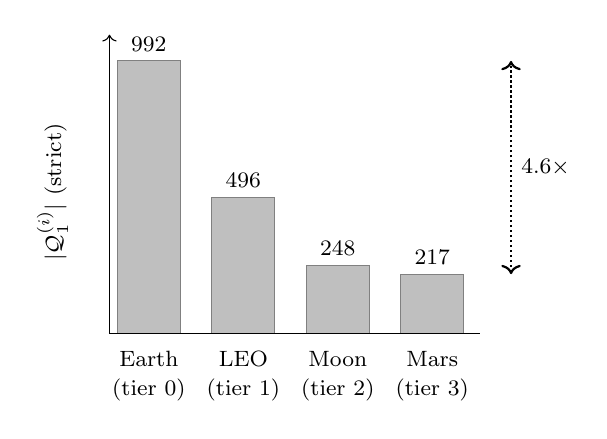
\begin{tikzpicture}[
    bar/.style={fill=black!25, draw=black!50},
    barlab/.style={font=\footnotesize, anchor=south},
    ticklab/.style={font=\footnotesize},
]
% Bars (scaled: max 992, chart height ~3.5cm)
\def\scale{0.0035}
\fill[bar] (0, 0) rectangle (0.8, 992*\scale);
\fill[bar] (1.2, 0) rectangle (2.0, 496*\scale);
\fill[bar] (2.4, 0) rectangle (3.2, 248*\scale);
\fill[bar] (3.6, 0) rectangle (4.4, 217*\scale);

% Bar labels (counts)
\node[barlab] at (0.4, 992*\scale) {992};
\node[barlab] at (1.6, 496*\scale) {496};
\node[barlab] at (2.8, 248*\scale) {248};
\node[barlab] at (4.0, 217*\scale) {217};

% X axis labels
\node[ticklab, anchor=north] at (0.4, -0.1) {Earth};
\node[ticklab, anchor=north] at (1.6, -0.1) {LEO};
\node[ticklab, anchor=north] at (2.8, -0.1) {Moon};
\node[ticklab, anchor=north] at (4.0, -0.1) {Mars};
\node[font=\footnotesize, anchor=north] at (0.4, -0.45) {(tier 0)};
\node[font=\footnotesize, anchor=north] at (1.6, -0.45) {(tier 1)};
\node[font=\footnotesize, anchor=north] at (2.8, -0.45) {(tier 2)};
\node[font=\footnotesize, anchor=north] at (4.0, -0.45) {(tier 3)};

% Y axis
\draw[->] (-0.1, 0) -- (-0.1, 3.8);
\node[font=\footnotesize, rotate=90, anchor=south] at (-0.5, 1.8) {$|\mathcal{Q}_1^{(i)}|$ (strict)};

% Axis line
\draw (-0.1, 0) -- (4.6, 0);

% 4.6x annotation
\draw[<->, thick, densely dotted] (5.0, 217*\scale) -- node[right, font=\footnotesize] {4.6$\times$} (5.0, 992*\scale);
\end{tikzpicture}
\caption{Phase~1 quorum count by initiating tier (strict $\mathcal{Q}_2$, from exhaustive TLA+ enumeration). Leadership flexibility increases monotonically from top to bottom of the wall.}
\label{fig:gradient}
\end{figure}

WPaxos~\cite{ailijiang2019wpaxos} uses symmetric grid quorums with uniform $Q_1$ structure regardless of initiator. By contrast, the wall uses tier-indexed families $\mathcal{Q}_1^{(i)}$, so partition failover cost is topology-proportional: if the leader is on Earth and Mars disconnects, leader election remains Earth-scoped.

\textbf{Terrestrial mapping, as a prediction.} The same structure appears wherever topology creates latency asymmetry: a cloud region as anchor, metro edge above it, a remote site above that; or disconnected, intermittent, low-bandwidth networks reachable only through windowed links. What makes these more than analogies is the direction of the pressure. Every latency economy argues for shrinking the commit quorum so the hot path stays local, and by the criterion of Section~\ref{sec:capability} that is precisely the direction which opens the commit-capable-but-acquisition-incapable state. Under our modeled retry policy that is the measured-harmful direction, but the terrestrial consequence remains a prediction. We state the status plainly: it is an argument from structure, not an evaluated result. Every claim in this paragraph is a hypothesis our criterion makes precise, and testing it on terrestrial topologies is future work.

\textbf{Future work.} The separation principle suggests three natural extensions: scoped write leases, where the anchor tier delegates write authority to upper tiers over bounded slot ranges---lease expiry on disconnection, conflict resolution via MRDTs/CRDTs---so that topology-scoped consistency becomes a managed contract rather than a binary cutoff; structured multi-anchor families that trade part of the linear readout for tolerance of anchor-tier partition (Section~\ref{sec:discussion}); and empirical validation of the terrestrial mapping on edge/cloud topologies where the same decomposition applies but the latency asymmetry is less dramatic.


\section{Conclusion}

Phase symmetry once made acquisition and commit formability coincide; Flexible Paxos can spend that coincidence while preserving cross-phase safety. We give the exact predicate-level correspondence for what follows: ordered predicates admit one capability gap, incomparable predicates admit both, and a generic auditor supplies deterministic witnesses. In the wall case study no Phase~2 threshold closes both gaps at every tier. Its upper-tier participation obligations buy topology-legible authority at the price of residual exposure, while the measured consequences remain bounded to our registered single-decree experiment and retry policy.

Mars makes the conflation visible; distance does not create it. Wherever quorum geometry meets changing, structured connectivity, node health and node counts can disagree with the service capabilities operators actually need. State-aware mitigation begins by exposing acquisition and commit separately, then combining that structural state with fresh runtime authority and a deliberately chosen client contract.

\bibliographystyle{plain}
\bibliography{references}

\appendix
\section{Simulator Parameters}
\label{app:params}

\begin{table}[h]
\centering
\small
\caption{Simulator parameters.}
\label{tab:params}
\begin{tabular}{llp{0.32\linewidth}}
\toprule
Parameter & Value & Notes \\
\midrule
Earth cross-cont.\ delay & 30--120~ms & per link pair \\
LEO--ground delay & 20--45~ms & per ground station \\
Moon one-way delay & 1.28~s & fixed \\
Mars one-way delay & 186--1342~s & swept \\
Mars-local delay & 5~ms & fixed \\
Processing delay & 1~ms & per acceptor \\
Jitter & $\pm$10\% & of link delay, uniform \\
Per-phase timeout & 500~s / 1~s & global / tier-local; global budget raised to $1.25\times$ the worst-case request--response path when that exceeds the base (above ${\approx}200$~s Mars delay) \\
Max Paxos rounds & 1 & per attempt \\
Blackout start & 600~s base & pre-window scaled to fit one full global round plus margin (930~s at 186~s Mars delay) \\
Simulation end & 4000~s base & horizon extends when pre/post windows scale \\
Reconciliation interval & 120~s & between global attempts \\
Loss model & none & deterministic link removal for blackout \\
\bottomrule
\end{tabular}
\end{table}

\section{Claim-to-Artifact Traceability}
\label{app:traceability}
Table~\ref{tab:traceability} maps the paper's main claims to executable artifacts. Paths are relative to the repository root of the (anonymized) artifact accompanying this submission. Results were generated with Python~$\ge$3.14 and SimPy~$\ge$4.1.1.

\begin{table*}[t]
\centering
\small
\caption{Claim-to-artifact traceability.}
\label{tab:traceability}
\begin{tabular}{p{0.28\linewidth}p{0.30\linewidth}p{0.34\linewidth}}
\toprule
Claim & Evidence & Artifact(s) \\
\midrule
Flat construction: 0\% during blackout at every hard-blackout sweep point. & Flat-mode sweep under the validated harness (\texttt{--global-quorum flat}). & \texttt{results/step9\_flat/\allowbreak step9\_sweep.csv}; \texttt{experiments/\allowbreak step9\_sweep.py}. \\
Majority baseline: 100\% during blackout, 361~ms two-phase decision latency at every hard-blackout sweep point. & Majority-mode sweep under the validated harness (\texttt{--global-quorum majority}). & \texttt{results/step9\_maj/\allowbreak step9\_sweep.csv}; \texttt{experiments/\allowbreak step9\_sweep.py}. \\
Crumbling wall: 100\% during blackout at every hard-blackout sweep point, 183~ms two-phase decision latency. & All rows show 100\% during-blackout. & \texttt{results/step9/\allowbreak step9\_sweep.csv}; \texttt{experiments/\allowbreak step9\_sweep.py}. \\
Per-tier liveness: 3 of 4 tiers retain global consensus during blackout. & Per-tier sweep, both topologies. & \texttt{results/tier\_liveness/\allowbreak tier\_sweep\_full\_ci.csv}; \texttt{experiments/\allowbreak tier\_liveness\_sweep.py}. \\
Sparse topology: LEO drops to 0\%. & Sparse rows in per-tier sweep. & Same as above. \\
Weakest-link migration and coordinated relaxation. & Crash-tolerance sweep rows. & \texttt{results/step10/\allowbreak step10\_sweep\_ci.csv}; \texttt{experiments/\allowbreak step10\_sweep.py}. \\
TLA+ verification of quorum intersection. & Exhaustive enumeration, all four tiers $\times$ \{strict, $k{=}4$, $k{=}3$\} (27{,}921 states, complete). & \texttt{tla/\allowbreak QuorumIntersection.tla}; \texttt{tla/\allowbreak ExhaustiveIntersection.tla}. \\
Paxos agreement model-checked. & 67M states (reduced topology, all-tier Phase~1 family, complete). & \texttt{tla/\allowbreak PaxosSmall.tla}. \\
Per-tier capability map: which (Phase~1, Phase~2) capability states each tier holds under each connectivity regime. & Exhaustive per-scenario classification, including the degraded partial-capability states. & \texttt{results/capability/\allowbreak capability\_map.csv}; \texttt{experiments/\allowbreak capability\_map.py}. \\
Containment characterization (Prop.~2) and the $k \le \lceil |E|/2 \rceil$ boundary (Prop.~3). & Exhaustive enumeration, 5~$k$ $\times$ 4~tiers; containment evaluated as set containment over minimal $Q_2$, not as the reachability restatement; 0 disagreements. Predicate monotonicity verified, not assumed. & \texttt{results/capability/\allowbreak dual\_containment.csv}; \texttt{experiments/\allowbreak capability\_dual\_sweep.py}. \\
Exact four-way gap correspondence and construction-independent audit. & Proposition~\ref{prop:gap} and Corollary~\ref{cor:correspondence} are primary. Independent state enumeration rejects a mutated report; all 129{,}032 three-node family-pair/pinned-domain cases pass; 16 registered wall cases reconcile with 0 CSV disagreements. & \texttt{quorum\_audit.py}; \texttt{experiments/\allowbreak quorum\_audit.py}; \texttt{results/capability/\allowbreak quorum\_audit\_registered.json}. \\
Wall-specific capability readout. & Deterministic operational demonstration over one planetary and one structurally analogous edge input; not evaluation. Runtime authority remains unknown and service policy is not inferred. & \texttt{experiments/\allowbreak capability\_readout.py}; \texttt{examples/capability/\allowbreak planetary\_moon\_01.json}; \texttt{examples/capability/\allowbreak edge\_remote\_01.json}. \\
Uniform threshold corollary: $(1,0)$ reachable iff $q_1 < q_2$; $(0,1)$ iff $q_2 < q_1$. & 80 threshold configurations ($n = 3..7$, all valid $q_1/q_2$), 0 violations. & \texttt{results/capability/\allowbreak dual\_uniform.csv}; \texttt{experiments/\allowbreak capability\_dual\_sweep.py}. \\
Valence of the two capability states: $(1,0)$ indistinguishable from a healthy contender; $(0,1)$ prevented decision in 50 of 50 seeds at retry budget~8 under the modeled retry policy. & Pre-registered experiment, 5 arms $\times$ 4 retry budgets $\times$ 50 seeds; predictions, falsification criterion, and declared consequence of a null committed before the experiment code existed; two registered predictions falsified and kept. Output byte-identical across two runs. & \texttt{results/flip/\allowbreak flip\_map.csv}; \texttt{results/flip/\allowbreak flip\_sweep.csv}; \texttt{flip.py}; \texttt{experiments/\allowbreak flip\_sweep.py}; \texttt{experiments/\allowbreak flip\_verdict.py}. \\
Price of coincidence: 0 at odd $n$, 1 at even $n$; cost-minimal configurations cannot be phase-symmetric at even $n$. & Re-analysis of the threshold enumeration; post-hoc, not pre-registered, and labelled as such. & \texttt{results/capability/\allowbreak dual\_uniform.csv}; \texttt{experiments/\allowbreak capability\_dual\_sweep.py}. \\
Tier-gradient: no $k$ closes both capability states; $T_2$ and $T_3$ retain $(0,1)$ at every $k$. & Exhaustive enumeration over all $2^{10}$ connectivity states, every tier and $k$, reported under both colocated-acceptor readings. Output byte-identical across two runs. & \texttt{results/capability/\allowbreak dual\_gradient\_map.csv}; \texttt{experiments/\allowbreak capability\_dual\_sweep.py}. \\
\bottomrule
\end{tabular}
\end{table*}

\end{document}
